\documentclass[11pt,a4paper]{article}
\usepackage[a4paper,margin=2.1cm,top=2.2cm,bottom=2.3cm]{geometry}
\usepackage[T1]{fontenc}
\usepackage{newtxtext,newtxmath}
\usepackage{amsmath}
\usepackage{graphicx}
\usepackage{booktabs,multirow,array}
\usepackage[dvipsnames]{xcolor}
\usepackage[most]{tcolorbox}
\usepackage{enumitem}
\usepackage{caption}
\usepackage{microtype}
\usepackage{fancyhdr}
\usepackage[section]{placeins}
\usepackage[colorlinks=true,linkcolor=skviolet,urlcolor=skviolet,citecolor=skviolet]{hyperref}
\usepackage[capitalise,noabbrev]{cleveref}

% SegEvalKit palette
\definecolor{skviolet}{HTML}{6D3FD6}
\definecolor{skdeep}{HTML}{2E1766}
\definecolor{sklight}{HTML}{F5F1FE}
\definecolor{skmid}{HTML}{D6C7FB}
\definecolor{skteal}{HTML}{139A8A}
\definecolor{skorange}{HTML}{E2712F}
\definecolor{skink}{HTML}{1D1733}
\definecolor{skmuted}{HTML}{8A84A3}

% generated by make_report.py
\newcommand{\nCases}{901}
\newcommand{\nCasesTS}{901}
\newcommand{\nStructures}{17}
\newcommand{\sekVersion}{0.1.0}
\newcommand{\evalDate}{2026-09-30}
\newcommand{\nsdTol}{2}
\newcommand{\minLesionVox}{10}
\newcommand{\connectivity}{26}
\newcommand{\rsuperCommit}{fa8fdce}
\newcommand{\rsuperDate}{2026-09-24}
\newcommand{\nPatched}{25}
\newcommand{\nPatchedZ}{23}
\newcommand{\nPatchedX}{2}
\newcommand{\nAuditCases}{227}
\newcommand{\nAuditFiles}{381}
\newcommand{\nAuditAorta}{218}
\newcommand{\auditSameShape}{all}
\newcommand{\mfPancDice}{.864}
\newcommand{\mfPancDiceMed}{.910}
\newcommand{\mfPancNSD}{.854}
\newcommand{\mfPancNSDMed}{.911}
\newcommand{\mfPancHD}{19.5}
\newcommand{\mfPancHDMed}{2.9}
\newcommand{\mfLiverDice}{.971}
\newcommand{\mfLiverDiceMed}{.981}
\newcommand{\mfLiverNSD}{.929}
\newcommand{\mfLiverNSDMed}{.961}
\newcommand{\mfLiverHD}{7.8}
\newcommand{\mfLiverHDMed}{1.9}
\newcommand{\mfSpleenDice}{.928}
\newcommand{\mfSpleenDiceMed}{.972}
\newcommand{\mfSpleenNSD}{.923}
\newcommand{\mfSpleenNSDMed}{.988}
\newcommand{\mfSpleenHD}{31.7}
\newcommand{\mfSpleenHDMed}{1.5}
\newcommand{\mfKidLDice}{.889}
\newcommand{\mfKidLDiceMed}{.966}
\newcommand{\mfKidLNSD}{.880}
\newcommand{\mfKidLNSDMed}{.970}
\newcommand{\mfKidLHD}{45.4}
\newcommand{\mfKidLHDMed}{1.8}
\newcommand{\mfDuodDice}{.897}
\newcommand{\mfDuodDiceMed}{.925}
\newcommand{\mfDuodNSD}{.910}
\newcommand{\mfDuodNSDMed}{.942}
\newcommand{\mfDuodHD}{15.6}
\newcommand{\mfDuodHDMed}{2.5}
\newcommand{\mfLesDice}{.597}
\newcommand{\mfLesDiceMed}{1.000}
\newcommand{\mfLesNSD}{.590}
\newcommand{\mfLesNSDMed}{1.000}
\newcommand{\mfLesHD}{206.5}
\newcommand{\mfLesHDMed}{0.0}
\newcommand{\mfCBDDice}{.643}
\newcommand{\mfCBDDiceMed}{.730}
\newcommand{\mfCBDNSD}{.768}
\newcommand{\mfCBDNSDMed}{.889}
\newcommand{\mfCBDHD}{128.4}
\newcommand{\mfCBDHDMed}{5.8}
\newcommand{\mfNOrgansAbove}{11}
\newcommand{\mfNOrgans}{16}
\newcommand{\mfGallMacro}{.805}
\newcommand{\mfGallPooled}{.879}
\newcommand{\mfPancPooled}{.855}
\newcommand{\nRefLesions}{161}
\newcommand{\nRefDetected}{131}
\newcommand{\mfLesDicePos}{.536}
\newcommand{\mfLesDiceNeg}{.609}
\newcommand{\mfNegNoPred}{457}
\newcommand{\nPosPatients}{151}
\newcommand{\nNegPatients}{750}
\newcommand{\mfLesSens}{0.81}
\newcommand{\mfLesPrec}{0.24}
\newcommand{\mfLesFone}{0.36}
\newcommand{\mfFPScan}{0.49}
\newcommand{\mfLesPooledDice}{0.55}
\newcommand{\mfAUC}{0.905}
\newcommand{\mfSens}{0.788}
\newcommand{\mfSpec}{0.900}
\newcommand{\mfThr}{0.96}
\newcommand{\mfNegFP}{0.52}
\newcommand{\mfPosLesRecall}{.836}
\newcommand{\mfPosLesFone}{.771}
\newcommand{\mfPosLesPrec}{.821}
\newcommand{\mfDetSmall}{4}
\newcommand{\mfDetBig}{97}
\newcommand{\nSmallLes}{25}
\newcommand{\mfECE}{0.040}
\newcommand{\mfBrier}{0.043}
\newcommand{\mfAUPRC}{0.640}
\newcommand{\nCompSig}{30}
\newcommand{\nComp}{30}
\newcommand{\maxPadj}{$<\!10^{-3}$}
\newcommand{\fracDiceMin}{79}
\newcommand{\fracDiceMax}{98}
\newcommand{\fracSpleenDice}{79}
\newcommand{\tsSpleenDice}{.946}
\newcommand{\tsSpleenHD}{7.6}
\newcommand{\tsSpleenHDMed}{1.6}
\newcommand{\tsPancDice}{.823}
\newcommand{\nHDmeanWorse}{7}
\newcommand{\nHDmedBetterFrac}{10}
\newcommand{\rankFlips}{spleen and the kidney (left)}
\newcommand{\nRankFlips}{2}
\newcommand{\tailSpleenN}{79}
\newcommand{\tailSpleenShare}{94}
\newcommand{\tailSpleenRefEmpty}{29}
\newcommand{\tailSpleenBoth}{50}
\newcommand{\tailSpleenBothDice}{.957}
\newcommand{\tailSpleenBothHD}{180}
\newcommand{\tsTailSpleenN}{14}
\newcommand{\refEmptySpleen}{55}
\newcommand{\mfPredOnEmptySpleen}{29}
\newcommand{\tsPredOnEmptySpleen}{1}
\newcommand{\tailKidLN}{101}
\newcommand{\tailKidLShare}{93}
\newcommand{\tailKidLRefEmpty}{47}
\newcommand{\tailKidLBoth}{53}
\newcommand{\tailKidLBothDice}{.953}
\newcommand{\tailKidLBothHD}{224}
\newcommand{\tsTailKidLN}{25}
\newcommand{\refEmptyKidL}{68}
\newcommand{\mfPredOnEmptyKidL}{47}
\newcommand{\tsPredOnEmptyKidL}{10}
\newcommand{\cohVenous}{.884}
\newcommand{\cohNoncon}{.806}
\newcommand{\cohGE}{.719}
\newcommand{\cohSiemens}{.850}
\newcommand{\cohThin}{.793}
\newcommand{\cohThick}{.894}
\newcommand{\cohPhaseP}{$<\!10^{-3}$}
\newcommand{\nCohSig}{25}
\newcommand{\nCohTests}{63}


\color{skink}
\setlength{\parindent}{0pt}
\setlength{\parskip}{4pt}
\setlength{\emergencystretch}{2.5em}
\captionsetup{font=small,labelfont={bf,color=skdeep},skip=4pt}
\setlist{itemsep=1pt,topsep=2pt,leftmargin=1.3em}
\renewcommand{\arraystretch}{1.12}

\pagestyle{fancy}
\fancyhf{}
\renewcommand{\headrulewidth}{0.4pt}
\renewcommand{\headrule}{\hbox to\headwidth{\color{skmid}\leaders\hrule height \headrulewidth\hfill}}
\fancyhead[L]{\small\color{skmuted}R-Super MedFormer on PanTS}
\fancyhead[R]{\small\color{skmuted}SegEvalKit \sekVersion}
\fancyfoot[C]{\small\color{skmuted}\thepage}

\makeatletter
\renewcommand\section{\@startsection{section}{1}{\z@}{-2.2ex plus -1ex minus -.2ex}{1.1ex}{\normalfont\Large\bfseries\color{skdeep}}}
\renewcommand\subsection{\@startsection{subsection}{2}{\z@}{-1.6ex plus -1ex minus -.2ex}{0.6ex}{\normalfont\large\bfseries\color{skviolet}}}
\makeatother

% boxes
\newtcolorbox{keybox}[1][]{enhanced,colback=sklight,colframe=skviolet,boxrule=0.6pt,arc=2pt,
  left=6pt,right=6pt,top=4pt,bottom=4pt,fonttitle=\bfseries,coltitle=white,colbacktitle=skviolet,#1}
\newtcolorbox{notebox}[1][]{enhanced,colback=white,colframe=skmid,boxrule=0.6pt,arc=2pt,
  left=6pt,right=6pt,top=3pt,bottom=3pt,#1}
% \metric{name}{formula}{kid explanation}{good values}{tiny example}
\newcommand{\metric}[5]{%
\begin{tcolorbox}[enhanced,breakable=false,colback=white,colframe=skmid,boxrule=0.6pt,arc=2pt,
  left=6pt,right=6pt,top=3pt,bottom=4pt,title={#1},fonttitle=\bfseries\small,coltitle=skdeep,
  colbacktitle=sklight,toptitle=1pt,bottomtitle=1pt]
\small
\begin{minipage}[t]{0.40\linewidth}\vspace{0pt}\centering #2\end{minipage}\hfill
\begin{minipage}[t]{0.57\linewidth}\vspace{0pt}
\textcolor{skviolet}{\textbf{Like you're 10:}} #3\par\smallskip
\textcolor{skviolet}{\textbf{Good values:}} #4\par\smallskip
\textcolor{skviolet}{\textbf{Tiny example:}} #5
\end{minipage}
\end{tcolorbox}}

\newcommand{\bignum}[2]{\begin{tabular}{@{}c@{}}{\fontsize{19}{21}\selectfont\bfseries\color{skviolet}#1}\\[1pt]{\footnotesize\color{skmuted}#2}\end{tabular}}

\begin{document}

% ------------------------------------------------------------------ title block
\begin{tcolorbox}[enhanced,colback=skdeep,colframe=skdeep,arc=3pt,left=10pt,right=10pt,top=8pt,bottom=8pt]
\color{white}
{\LARGE\bfseries Evaluating the R-Super MedFormer model on PanTS}\par\smallskip
{\large with the SegEvalKit evaluation library}\par\medskip
{\small \nCases{} test CT scans \textbullet{} \nStructures{} structures \textbullet{} organ, tumour and patient-level metrics
\textbullet{} evaluated \evalDate{} with SegEvalKit \sekVersion}
\end{tcolorbox}

\section*{At a glance}

\begin{keybox}[title={What we tested}]
\small
\begin{tabular}{@{}>{\bfseries}p{2.4cm}p{12.9cm}@{}}
Model & \textbf{MedFormer}, the segmentation model of the \textbf{R-Super} project (Report Supervision, Johns Hopkins University).
  This is the only R-Super model we ran. It is the public checkpoint \texttt{AbdomenAtlas/MedFormerPanTS}, which the
  authors describe as their ``segmentation'' baseline, trained on the PanTS public dataset; the report-supervised
  R-Super models were not evaluated here. \\
Code & Official R-Super repository (\texttt{MrGiovanni/R-Super}, commit \texttt{\rsuperCommit}, \rsuperDate), official
  inference script \texttt{predict\_abdomenatlas.py}, with one disclosed bug fix (\cref{sec:fix}). \\
Dataset & \textbf{PanTS} (Pancreatic Tumor Segmentation dataset), public \textbf{test split}: \nCases{} contrast and
  non-contrast abdominal CTs with expert per-structure masks and patient metadata. \\
Comparator & TotalSegmentator v2 (\texttt{total} task), a widely used general model, as a reference point only. \\
Evaluation & SegEvalKit \sekVersion: every metric on every case, then test-set, patient-level, paired and cohort
  statistics. Every number in this report is generated from the evaluation output files.
\end{tabular}
\end{keybox}

\vspace{2pt}
\begin{center}
\begin{tabular}{cccccc}
\bignum{\mfPancDice}{pancreas Dice} & \bignum{\mfLiverDice}{liver Dice} & \bignum{\mfPancHDMed\,mm}{pancreas HD95 (median)} &
\bignum{\mfAUC}{tumour yes/no AUC} & \bignum{\mfLesSens}{tumours found} & \bignum{\mfFPScan}{false tumours / scan}
\end{tabular}
\end{center}
\vspace{-2pt}

\begin{keybox}[title={Five things the numbers say}]
\small
\begin{enumerate}[leftmargin=1.4em]
\item \textbf{Strong organ segmentation.} MedFormer's mean Dice is at least 0.85 on \mfNOrgansAbove{} of its
  \mfNOrgans{} organs and vessels (pancreas \mfPancDice, median \mfPancDiceMed). On the ten organs it shares with
  TotalSegmentator it has the higher Dice in \fracDiceMin\% to \fracDiceMax\% of the patients.
\item \textbf{A few cases drive the average boundary error.} On the spleen, \tailSpleenN{} of \nCases{} cases with an
  HD95 above 50\,mm make up \tailSpleenShare\% of the mean HD95 (median \mfSpleenHDMed\,mm, mean \mfSpleenHD\,mm).
  \tailSpleenRefEmpty{} of them are patients with no reference spleen mask in which MedFormer still predicts a spleen;
  the other \tailSpleenBoth{} are good segmentations (median Dice \tailSpleenBothDice) with some predicted voxels far
  from the organ.
\item \textbf{How you rank decides who wins.} On the \rankFlips, ranking by mean Dice puts TotalSegmentator first,
  while counting in how many patients each model is better puts MedFormer first.
\item \textbf{Tumours: sensitive, not precise.} At the patient level MedFormer separates patients with and without a
  pancreatic tumour with an AUC of \mfAUC. It finds \mfLesSens{} of all \nRefLesions{} reference tumours, but only
  \mfLesPrec{} of its predicted tumours match a real one (\mfFPScan{} false tumours per scan), and tumours smaller than
  0.5\,mL are almost always missed (\mfDetSmall\% of \nSmallLes).
\item \textbf{Performance depends on the scan.} Pancreas Dice is \cohVenous{} on venous-phase and \cohNoncon{} on
  non-contrast scans, and \cohSiemens{} on Siemens against \cohGE{} on GE scanners; \nCohSig{} of \nCohTests{} cohort
  tests are significant after correction.
\end{enumerate}
\end{keybox}

\newpage
% ------------------------------------------------------------------
\section{What we tested, and how}
\label{sec:setup}

\subsection{The model: MedFormer from R-Super}
R-Super (Report Supervision) is a method from Johns Hopkins University that trains tumour segmentation models with
radiology reports in addition to masks (Bassi \emph{et al.}, MICCAI 2025). Its repository releases a MedFormer model
trained with masks on PanTS, the checkpoint \texttt{AbdomenAtlas/MedFormerPanTS}, which its model card calls the
public ``segmentation'' baseline and the starting point for report supervision. We evaluate \emph{this} checkpoint
(\texttt{pants\_pancreas\_release/fold\_0\_latest.pth}), the only R-Super model we ran. It predicts 26 classes,
including the pancreas, its head, body and tail, the pancreatic lesion and the surrounding organs and vessels, and it
writes lesion probabilities.

We ran the official script \texttt{predict\_abdomenatlas.py} on NVIDIA A100 GPUs of the MBZUAI DANA cluster, as
SLURM batch jobs (\texttt{benchmarks/pants/run\_medformer.sbatch}), with the options
\begin{center}\small\texttt{--organ\_mask\_on\_lesion\ \ --save\_probabilities\_lesions\ \ --organs\_with\_tumor pancreas}\end{center}

\subsection{One fix to the official code}
\label{sec:fix}
\begin{notebox}
\small
\textbf{What went wrong.} On \nPatched{} of the \nCases{} scans the official script finished the network prediction but
failed when writing the result. The cause is in \texttt{pad\_to\_training\_size}: PyTorch's \texttt{F.pad} lists the
\emph{last} axis first, so a scan with fewer than 128 voxels along one axis (after resampling to 1\,mm) is padded along
the wrong axis while the offsets are recorded for the right one. Removing the padding then cuts the wrong axis and the
output no longer matches the CT (\nPatchedZ{} scans short along $z$, \nPatchedX{} narrow along $x$).\\
\par\raggedright\textbf{What we did.} We ran a copy of the script with the two padding lines swapped
(\texttt{benchmarks/pants/patch\_medformer.py}); the official file is unchanged. The fixed lines only run for such
small scans, so the other \the\numexpr\nCases-\nPatched\relax{} predictions are identical with and without the fix.
\end{notebox}

\subsection{The data: PanTS test split}
PanTS is a public CT dataset of the pancreas and pancreatic tumours. Its test split has \nCases{} CT scans, of which
\nPosPatients{} contain a pancreatic tumour and \nNegPatients{} do not. Each scan comes with one mask file per
structure, and a metadata table gives the CT phase, scanner, site country, slice thickness, sex and age.

We evaluate \nStructures{} structures: the pancreas, the pancreatic lesion, liver, spleen, both kidneys, stomach,
gallbladder, duodenum, colon, both adrenal glands, aorta, inferior vena cava, superior mesenteric artery, veins and
common bile duct.

\begin{notebox}
\small
\textbf{Two dataset details that change the numbers.}
\begin{itemize}
\item \textbf{Pancreas = pancreas + tumour.} In PanTS the tumour mask is not always inside the pancreas mask, so the
  pancreas is scored as the union of the two, on both the reference and the prediction.
\item \textbf{Unreliable label headers.} \texttt{segevalkit audit} finds that in \nAuditCases{} of the \nCases{} scans
  at least one reference mask (\nAuditFiles{} files, \nAuditAorta{} of them aortas) stores an orientation or origin
  that disagrees with its CT, although its voxels line up with the CT and \auditSameShape{} of them have the CT's
  shape. Aligning masks by their headers would move correct predictions out of place, so every mask is compared
  voxel by voxel with the CT grid.
\end{itemize}
\end{notebox}

\subsection{The evaluation protocol}
\begin{itemize}
\item Organs: Dice, IoU, NSD at \nsdTol\,mm, HD95, ASSD, MASD, precision, recall and volume errors. Tubular
  structures (aorta, vena cava, veins, arteries, bile duct) also get clDice and Betti errors.
\item Pancreatic lesion: the organ metrics plus lesion-level detection (tumours are connected blobs,
  \connectivity-connectivity, blobs under \minLesionVox{} voxels ignored), panoptic quality, lesion counts and
  probability calibration.
\item Empty masks: if both reference and prediction are empty the case is perfect (Dice 1, HD95 0); if only one is
  empty, overlap scores are 0 and distances are the image diagonal. A missing prediction counts as empty.
\item Test set: per-case means with 95\% bootstrap intervals, pooled (voxel-summed) values, patient-level tumour
  detection, paired tests against TotalSegmentator, two ranking schemes and cohort tests on the metadata.
\end{itemize}
PanTS does not publish its evaluation script, NSD tolerance or detection rule, so these numbers follow the documented
SegEvalKit protocol and are not directly comparable with the PanTS leaderboard.

% ------------------------------------------------------------------
\section{How each metric works, explained simply}
\label{sec:metrics}

\begin{keybox}[title={The picture game}]
\small
A CT scan is a big 3D picture made of tiny cubes called \emph{voxels}. Doctors coloured the cubes that belong to,
say, the pancreas: that is the \textbf{answer key} (the \emph{reference}, $G$). The model coloured its own guess:
the \textbf{prediction} $P$. Comparing the two gives three counts:
\textcolor{skviolet}{\textbf{TP}} (coloured by both), \textcolor{skteal}{\textbf{FP}} (coloured by the model only,
extra) and \textcolor{skorange}{\textbf{FN}} (in the answer, but missed). Every overlap metric is built from these.\par
\begin{center}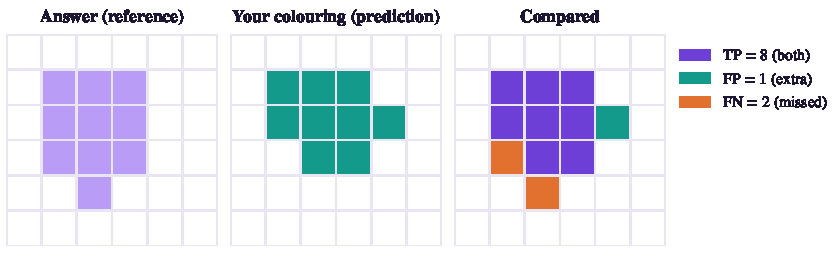
\includegraphics[width=0.84\linewidth]{figures/f_toy_grid.pdf}\end{center}
\vspace{-4pt}
The examples below use this picture: the answer has 10 squares, the colouring has 9, and 8 are shared, so
TP\,=\,8, FP\,=\,1, FN\,=\,2.
\end{keybox}

\subsection{Overlap: how much of the shape is right?}

\metric{Dice similarity coefficient (DSC)}
{$\displaystyle \mathrm{DSC}=\frac{2\,TP}{2\,TP+FP+FN}$}
{Count the shared squares twice and divide by all the squares coloured in both pictures. It is the most common
segmentation score.}
{0 (no overlap) to 1 (perfect). Higher is better.}
{$2\cdot 8/(2\cdot 8+1+2)=16/19=0.84$.}

\metric{Intersection over union (IoU)}
{$\displaystyle \mathrm{IoU}=\frac{TP}{TP+FP+FN}$}
{Shared squares divided by all squares that anyone coloured. It is always a bit lower than Dice and tells the same
story.}
{0 to 1. Higher is better.}
{$8/(8+1+2)=8/11=0.73$.}

\metric{Precision and recall}
{$\displaystyle \mathrm{Precision}=\frac{TP}{TP+FP}$\\[4pt]$\displaystyle \mathrm{Recall}=\frac{TP}{TP+FN}$}
{Precision: of the squares you coloured, how many were right? Recall: of the squares you should have coloured, how
many did you colour? A model that colours too much has low precision; one that colours too little has low recall.}
{0 to 1. Higher is better.}
{Precision $8/9=0.89$; recall $8/10=0.80$.}

\metric{Relative volume difference (RVD)}
{$\displaystyle \mathrm{RVD}=\frac{|P|-|G|}{|G|}$}
{Is the amount right? Compare the number of coloured squares with the answer, as a fraction. It ignores
\emph{where} the squares are.}
{0 is perfect; $-0.2$ means 20\% too small, $+0.2$ means 20\% too big.}
{$(9-10)/10=-0.10$: 10\% too small.}

\subsection{Boundary: where is the outline wrong, in millimetres?}
For these metrics we take the outline (surface) of each shape and measure, for every point of one outline, the
distance in millimetres to the closest point of the other outline: $D_{P\to G}$ from the prediction to the reference
and $D_{G\to P}$ back.

\metric{Normalised surface Dice (NSD at $\tau$ = \nsdTol\,mm)}
{$\displaystyle \mathrm{NSD}_\tau=\frac{N_\tau(D_{P\to G})+N_\tau(D_{G\to P})}{|\partial P|+|\partial G|}$\\[3pt]
{\footnotesize $N_\tau$ counts the distances $\le\tau$; $|\partial P|$, $|\partial G|$ are the numbers of outline points}}
{Draw a 2\,mm ``safe zone'' along each outline. NSD is the fraction of both outlines that lies inside the other's
safe zone. Small wobbles are forgiven; real boundary mistakes are not.}
{0 to 1. Higher is better.}
{Each outline has 20 points; 17 of the prediction's and 18 of the reference's are within 2\,mm:
$(17+18)/40=0.875$.}

\metric{95th-percentile Hausdorff distance (HD95)}
{$\displaystyle \mathrm{HD}_{95}=\max\big(P_{95}(D_{P\to G}),\,P_{95}(D_{G\to P})\big)$}
{Line up all the outline distances from nearest to farthest. HD95 is the distance that 95\% of the points are
within, taken in the worse direction. It ignores the worst 5\% so one stray point does not decide the score, but if
more than 5\% of the outline is far away, HD95 becomes large.}
{0\,mm is perfect. Lower is better. If one mask is empty, HD95 is the size of the whole image (hundreds of mm).}
{100 outline points: 96 are within 1\,mm and 4 are 30\,mm away, so HD95 is 1\,mm. With 10 points at 30\,mm,
HD95 is 30\,mm.}

\metric{Average symmetric surface distance (ASSD)}
{$\displaystyle \mathrm{ASSD}=\frac{\sum D_{P\to G}+\sum D_{G\to P}}{|\partial P|+|\partial G|}$}
{The average distance between the two outlines, using every point of both.}
{0\,mm is perfect. Lower is better.}
{Prediction points 0, 1, 1, 2\,mm away; reference points 1, 1, 0, 0\,mm: $(4+2)/8=0.75$\,mm.}

\subsection{Tumours: were they found, and only them?}
Tumours are counted as blobs (connected groups of voxels). A reference tumour is \emph{found} if any predicted blob
touches it; a predicted blob that touches no real tumour is a \emph{false tumour}.

\metric{Lesion sensitivity, precision and F1}
{$\displaystyle \mathrm{Sens}=\frac{TP_{\mathrm{les}}}{TP_{\mathrm{les}}+FN_{\mathrm{les}}}$\\[4pt]
$\displaystyle \mathrm{Prec}=\frac{TP_{\mathrm{les}}}{TP_{\mathrm{les}}+FP_{\mathrm{les}}}$\\[4pt]
$\displaystyle \mathrm{F1}=\frac{2\,TP_{\mathrm{les}}}{2\,TP_{\mathrm{les}}+FP_{\mathrm{les}}+FN_{\mathrm{les}}}$}
{Hide and seek: sensitivity is how many hidden friends you found; precision is how often you were right when you
shouted ``found you!''; F1 combines both.}
{0 to 1. Higher is better.}
{4 real tumours, 3 found: sensitivity $3/4=0.75$. 5 predicted blobs, 3 on a real tumour: precision $3/5=0.60$.
F1 $=6/(6+2+1)=0.67$.}

\metric{False-positive lesions per scan}
{$\displaystyle \frac{\sum_{\text{scans}} FP_{\mathrm{les}}}{\text{number of scans}}$}
{On average, how many false alarms does a doctor see per scan?}
{0 is perfect. Lower is better.}
{5 false blobs over 10 scans: 0.5 per scan.}

\metric{Lesion-wise Dice and panoptic quality (PQ)}
{$\displaystyle \mathrm{LW\text{-}DSC}=\frac{\sum_{i}\mathrm{DSC}_i}{N_G+FP_{\mathrm{les}}}$\\[4pt]
$\displaystyle \mathrm{PQ}=\underbrace{\tfrac{\sum \mathrm{IoU}}{|TP|}}_{\text{shape}}\times
\underbrace{\tfrac{|TP|}{|TP|+\frac12|FP|+\frac12|FN|}}_{\text{finding}}$}
{Lesion-wise Dice scores every tumour separately, so a small tumour counts as much as a big one; missed and false
tumours score 0. PQ multiplies ``how well are the found tumours shaped'' by ``how well were tumours found'' (a
match needs IoU above 0.5).}
{0 to 1. Higher is better.}
{Two tumours, Dice 0.8 and 0 (missed), plus one false blob: $0.8/3=0.27$. PQ with matches of IoU 0.8 and 0.6,
one false and one missed: $0.7\times 2/3=0.47$.}

\metric{Patient level: sensitivity, specificity and AUC}
{$\displaystyle \mathrm{Sens}=\frac{\text{sick patients flagged}}{\text{sick patients}}$\\[4pt]
$\displaystyle \mathrm{Spec}=\frac{\text{healthy not flagged}}{\text{healthy patients}}$\\[4pt]
AUC $=$ area under the curve of Sens vs.\ $1-$Spec over all thresholds}
{The doctor's question: does this patient have a tumour? The model says ``yes'' if its predicted tumour volume is above
a threshold. The AUC is the chance that a random sick patient gets a larger predicted tumour than a random healthy
one. We report sensitivity at the smallest threshold with specificity at least 0.90.}
{0.5 is guessing, 1 is perfect. Higher is better.}
{10 sick patients, 8 flagged: sensitivity 0.8. 20 healthy, 18 not flagged: specificity 0.9.}

\subsection{Probabilities: can the model's confidence be trusted?}
MedFormer also writes a probability for every voxel of being tumour. These metrics use the voxels within 10\,mm of
either mask.

\metric{Expected calibration error (ECE)}
{$\displaystyle \mathrm{ECE}=\sum_{b=1}^{B}\frac{|B_b|}{N}\big|\mathrm{acc}(B_b)-\mathrm{conf}(B_b)\big|$}
{Like a weather forecaster: when they say ``90\% sure'', it should be right 9 times out of 10. Group voxels by how
sure the model is ($B=15$ groups), and average the gap between how sure it was and how often it was right.}
{0 is perfectly honest. Lower is better.}
{100 voxels at 90\% confidence, 80 correct: gap 0.10. If every group looks like this, ECE is 0.10.}

\metric{Brier score and area under the precision--recall curve}
{$\displaystyle \mathrm{BS}=\frac1N\sum_i(p_i-g_i)^2$\\[4pt]
$\displaystyle \mathrm{AP}=\sum_k (R_k-R_{k-1})\,P_k$}
{Brier: the average squared miss between the probability and the truth (1 tumour, 0 not). AP: sort voxels from most
to least suspicious and check whether the real tumour voxels come first; it only exists for patients with a tumour.}
{Brier 0 is perfect (lower is better); AP 1 is perfect (higher is better).}
{Probability 0.9 on a tumour voxel: $(0.9-1)^2=0.01$; on a healthy voxel: $0.9^2=0.81$; mean $0.41$.}

\subsection{From many patients to one conclusion}

\metric{Macro (per-patient) vs.\ pooled (per-voxel) averages}
{$\displaystyle \overline{\mathrm{DSC}}=\frac1n\sum_i \mathrm{DSC}_i$\\[4pt]
$\displaystyle \mathrm{DSC}_{\text{pooled}}=\frac{2\sum_i TP_i}{2\sum_i TP_i+\sum_i FP_i+\sum_i FN_i}$}
{Macro gives every patient one vote. Pooled throws all voxels of all patients into one bag, so big organs and big
tumours get more say.}
{Both 0 to 1. When they disagree, a few patients with small structures are failing.}
{Patient A: TP 900, FP 100, FN 100 (Dice 0.90). Patient B: a 10-voxel structure missed (Dice 0). Macro 0.45; pooled
$1800/2010=0.90$.}

\metric{Bootstrap 95\% confidence interval}
{resample the $n$ patients with replacement, recompute the mean, repeat 1000 times; the interval holds the middle
95\% of these means}
{If we had tested a different bag of 901 patients, how much could the average change? We fake many new bags by drawing
patients from our own bag (some twice, some not at all) and look at how much the average moves.}
{A narrow interval means a trustworthy average.}
{If the middle 95\% of 1000 resampled means runs from 0.85 to 0.87, the interval is [0.85, 0.87].}

\metric{Paired Wilcoxon test with Holm correction}
{$\displaystyle W^+=\sum_{d_i>0}\operatorname{rank}(|d_i|)$\\[4pt]
Holm: $\tilde p_{(k)}=\max_{j\le k}\min\big(1,(m-j+1)\,p_{(j)}\big)$}
{Both models take the same test on the same patients. For each patient we note who did better and by how much. If one
model wins more often \emph{and} by more, the test says it is not luck. Asking many questions at once makes some
look lucky by chance, so Holm raises the bar with every extra question.}
{A small adjusted $p$ (below 0.05) means a real difference; the \emph{fraction of patients where a model is better}
says how big it is.}
{Differences $+0.05,+0.02,-0.01,+0.04,+0.03$: ranks 5, 2, 1, 4, 3, so $W^+=14$, $W^-=1$, better in 4 of 5.
Holm on $p=0.01,0.02,0.04$ gives $0.03,0.04,0.04$.}

\begin{tcolorbox}[enhanced,colback=white,colframe=skmid,boxrule=0.6pt,arc=2pt,left=6pt,right=6pt,top=3pt,bottom=4pt,
  title={Two ways to rank models},fonttitle=\bfseries\small,coltitle=skdeep,colbacktitle=sklight,toptitle=1pt,bottomtitle=1pt]
\small
\begin{minipage}[c]{0.44\linewidth}\centering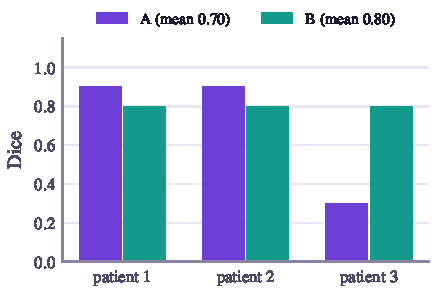
\includegraphics[width=\linewidth]{figures/f_toy_rank.pdf}\end{minipage}\hfill
\begin{minipage}[c]{0.53\linewidth}
\textcolor{skviolet}{\textbf{Aggregate-then-rank:}} average each model's scores, then rank the averages.
\textcolor{skviolet}{\textbf{Rank-then-aggregate:}} rank the models on each patient, then average the ranks.\par\smallskip
\textcolor{skviolet}{\textbf{Like you're 10:}} is the best runner the one with the best average time, or the one who
wins most races?\par\smallskip
\textcolor{skviolet}{\textbf{Tiny example:}} A scores 0.9, 0.9, 0.3 (mean 0.70); B scores 0.8 three times (mean 0.80).
By averages B wins. By races A wins twice: mean rank A $=(1+1+2)/3=1.33$, B $=1.67$, so A wins.
\end{minipage}
\end{tcolorbox}

\metric{Cohort tests: Kruskal--Wallis and Mann--Whitney}
{$\displaystyle H=\frac{12}{N(N+1)}\sum_{g}\frac{R_g^2}{n_g}-3(N+1)$\\[4pt]
effect size $\varepsilon^2=\dfrac{H-k+1}{N-k}$}
{Line up all patients from worst to best Dice. If one group (for example venous-phase scans) keeps standing near the
front, the groups differ. Two groups use the Mann--Whitney test, more groups the Kruskal--Wallis test ($R_g$ is the
sum of the places of group $g$).}
{Small adjusted $p$: the groups differ. The groups are observational, so a difference can come from other
differences between them (site, disease), not only the factor named.}
{Six patients in two groups taking places $\{1,2,3\}$ and $\{4,5,6\}$: $H=\tfrac{12}{42}(\tfrac{36}{3}+\tfrac{225}{3})-21=3.86$.}

% ------------------------------------------------------------------
\section{Results}
\label{sec:results}

\subsection{Organs and vessels}

\begin{table}[!htbp]
\centering\small
\caption{\textbf{MedFormer on the \nCases{} PanTS test CTs.} Mean with 95\% bootstrap interval, and median, per
structure. The pancreas includes the tumour; the lesion row averages over all patients, including tumour-free ones
(see \cref{sec:lesions}).}
\label{tab:structures}
\setlength{\tabcolsep}{4pt}
% generated by make_report.py
\begin{tabular}{lrrrrrr}
\toprule
 & \multicolumn{2}{c}{Dice $\uparrow$} & \multicolumn{2}{c}{NSD (\nsdTol\,mm) $\uparrow$} & \multicolumn{2}{c}{HD95 (mm) $\downarrow$} \\
 & mean [95\% CI] & median & mean [95\% CI] & median & mean [95\% CI] & median \\
\midrule
Pancreas & .864 {\scriptsize [.854, .874]} & .910 & .854 {\scriptsize [.842, .864]} & .911 & 19.5 {\scriptsize [15.3, 24.5]} & 2.9 \\
Pancreatic lesion & .597 {\scriptsize [.566, .626]} & 1.000 & .590 {\scriptsize [.558, .619]} & 1.000 & 206.5 {\scriptsize [188.4, 225.4]} & 0.0 \\
Liver & .971 {\scriptsize [.965, .975]} & .981 & .929 {\scriptsize [.921, .935]} & .961 & 7.8 {\scriptsize [5.7, 10.6]} & 1.9 \\
Spleen & .928 {\scriptsize [.915, .939]} & .972 & .923 {\scriptsize [.910, .935]} & .988 & 31.7 {\scriptsize [24.9, 39.6]} & 1.5 \\
Kidney (left) & .889 {\scriptsize [.872, .904]} & .966 & .880 {\scriptsize [.863, .895]} & .970 & 45.4 {\scriptsize [36.5, 55.0]} & 1.8 \\
Kidney (right) & .939 {\scriptsize [.929, .947]} & .969 & .928 {\scriptsize [.918, .937]} & .972 & 22.6 {\scriptsize [16.9, 28.3]} & 1.7 \\
Stomach & .903 {\scriptsize [.893, .913]} & .955 & .857 {\scriptsize [.846, .869]} & .925 & 16.9 {\scriptsize [14.0, 20.1]} & 2.8 \\
Gallbladder & .805 {\scriptsize [.788, .820]} & .913 & .823 {\scriptsize [.806, .838]} & .935 & 56.7 {\scriptsize [48.5, 66.0]} & 2.6 \\
Duodenum & .897 {\scriptsize [.890, .904]} & .925 & .910 {\scriptsize [.902, .918]} & .942 & 15.6 {\scriptsize [12.1, 19.8]} & 2.5 \\
Colon & .921 {\scriptsize [.915, .926]} & .942 & .899 {\scriptsize [.891, .905]} & .927 & 12.3 {\scriptsize [10.3, 14.9]} & 3.3 \\
Adrenal (left) & .837 {\scriptsize [.826, .848]} & .877 & .928 {\scriptsize [.916, .940]} & .982 & 54.4 {\scriptsize [46.8, 62.6]} & 1.5 \\
Adrenal (right) & .843 {\scriptsize [.834, .851]} & .874 & .940 {\scriptsize [.930, .949]} & .981 & 60.2 {\scriptsize [51.4, 68.9]} & 1.5 \\
Aorta & .903 {\scriptsize [.896, .909]} & .936 & .914 {\scriptsize [.906, .920]} & .948 & 15.0 {\scriptsize [13.2, 17.2]} & 2.7 \\
Inferior vena cava & .854 {\scriptsize [.845, .864]} & .913 & .853 {\scriptsize [.843, .862]} & .901 & 22.0 {\scriptsize [19.2, 25.4]} & 4.3 \\
Sup. mesenteric artery & .836 {\scriptsize [.828, .844]} & .863 & .947 {\scriptsize [.936, .955]} & .982 & 32.4 {\scriptsize [26.4, 39.2]} & 1.5 \\
Veins & .860 {\scriptsize [.852, .866]} & .890 & .922 {\scriptsize [.914, .928]} & .949 & 21.4 {\scriptsize [17.7, 25.7]} & 2.5 \\
Common bile duct & .643 {\scriptsize [.626, .659]} & .730 & .768 {\scriptsize [.749, .786]} & .889 & 128.4 {\scriptsize [117.7, 140.1]} & 5.8 \\
\bottomrule
\end{tabular}

\end{table}

\begin{figure}[!htbp]
\centering
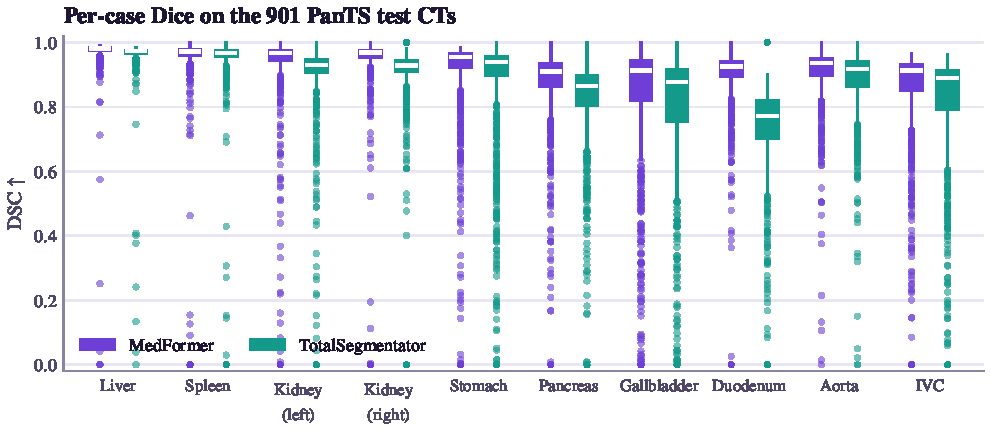
\includegraphics[width=\linewidth]{figures/f_dice_dist.pdf}
\caption{\textbf{Every patient, not just the average.} Per-case Dice of MedFormer and TotalSegmentator on the ten
shared organs (box: middle 50\% of patients, line: median, dots: outliers).}
\label{fig:dist}
\end{figure}

Medians are higher than means for almost every structure because a minority of patients score far below the rest
(\cref{fig:dist}). The mean HD95 in particular is dominated by a few cases:

\begin{figure}[!htbp]
\centering
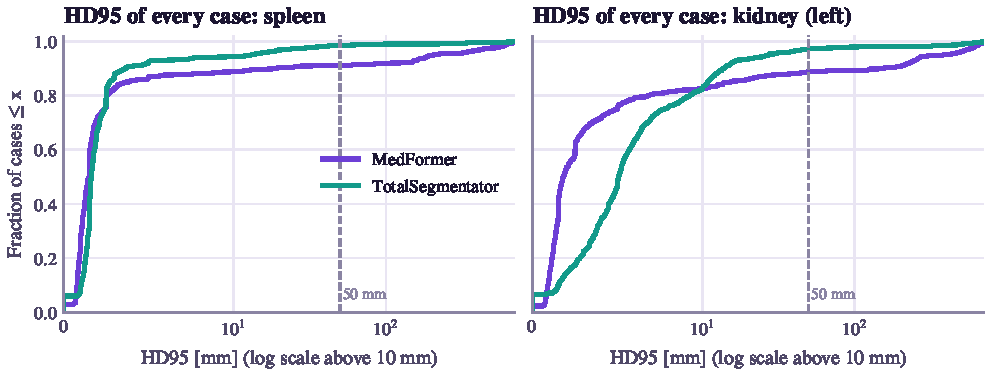
\includegraphics[width=\linewidth]{figures/f_hd95_tail.pdf}
\caption{\textbf{The HD95 failure tail.} Fraction of patients with HD95 up to $x$. Most MedFormer cases are within a
few millimetres, but about one in ten is far above 50\,mm (dashed).}
\label{fig:tail}
\end{figure}

\begin{notebox}
\small
\textbf{Where the tail comes from.} On the spleen, \tailSpleenN{} cases have an HD95 above 50\,mm and make up
\tailSpleenShare\% of the mean. In \tailSpleenRefEmpty{} of them the reference has no spleen mask but MedFormer predicts
one, which the empty-mask rule scores with the image diagonal (\refEmptySpleen{} test scans have an empty spleen mask;
MedFormer predicts a spleen in \mfPredOnEmptySpleen{} of them, TotalSegmentator in \tsPredOnEmptySpleen). The other
\tailSpleenBoth{} are good segmentations (median Dice \tailSpleenBothDice) with more than 5\% of the predicted outline
far from the organ (median HD95 \tailSpleenBothHD\,mm). The left kidney behaves the same way: \tailKidLN{} cases,
\tailKidLShare\% of the mean, \tailKidLRefEmpty{} with an empty reference.
\end{notebox}

\subsection{Macro vs.\ pooled}

\begin{table}[!htbp]
\centering\small
\caption{\textbf{Per-patient (macro) and per-voxel (pooled) Dice.} Pooled precision and recall show whether the model
tends to over- or under-segment.}
\label{tab:levels}
% generated by make_report.py
\begin{tabular}{lrrrr}
\toprule
Structure & macro Dice & pooled Dice & pooled precision & pooled recall \\
\midrule
Pancreas & .864 & .855 & .817 & .897 \\
Liver & .971 & .975 & .975 & .976 \\
Spleen & .928 & .965 & .962 & .967 \\
Kidney (left) & .889 & .936 & .919 & .955 \\
Kidney (right) & .939 & .951 & .944 & .959 \\
Stomach & .903 & .928 & .916 & .940 \\
Gallbladder & .805 & .879 & .836 & .927 \\
Duodenum & .897 & .905 & .910 & .900 \\
Colon & .921 & .933 & .946 & .921 \\
Adrenal (left) & .837 & .861 & .854 & .868 \\
Adrenal (right) & .843 & .852 & .842 & .862 \\
Aorta & .903 & .902 & .885 & .919 \\
Inferior vena cava & .854 & .877 & .845 & .911 \\
Sup. mesenteric artery & .836 & .849 & .847 & .852 \\
Veins & .860 & .875 & .876 & .874 \\
Common bile duct & .643 & .692 & .614 & .793 \\
\bottomrule
\end{tabular}

\end{table}

Where the two agree the model is consistent across patients; where pooled is higher (gallbladder \mfGallMacro{} macro
vs.\ \mfGallPooled{} pooled), a minority of small or unusual structures fails and pulls down the per-patient average.

\subsection{Pancreatic tumours}
\label{sec:lesions}

\begin{figure}[!htbp]
\centering
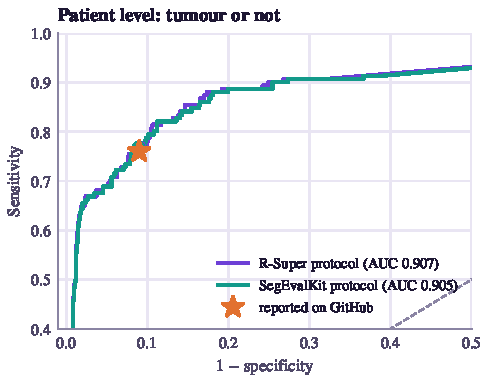
\includegraphics[width=0.49\linewidth]{figures/f_roc.pdf}\hfill
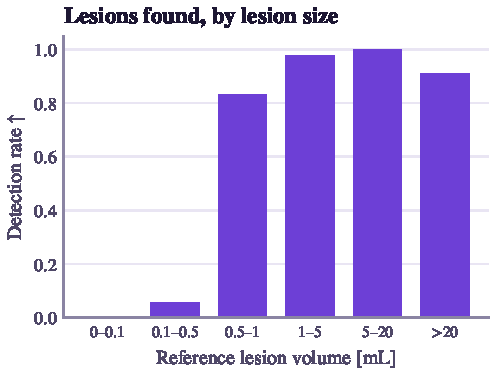
\includegraphics[width=0.49\linewidth]{figures/f_det_size.pdf}
\caption{\textbf{Patient-level and lesion-level detection.} Left: ROC curve of the predicted tumour volume as a
``tumour or not'' score over \nPosPatients{} patients with and \nNegPatients{} without a tumour; the dot is the
operating point at specificity $\ge$ 0.90 (threshold \mfThr\,mL). Right: fraction of reference tumours found, by
tumour size.}
\label{fig:det}
\end{figure}

\begin{table}[!htbp]
\centering\small
\caption{\textbf{Tumour detection.} Left: over the whole test set (\nRefLesions{} reference tumours; intervals
resample patients). Right: reference tumours found, by size.}
\label{tab:lesion}
\setlength{\tabcolsep}{4pt}\begin{tabular}{@{}c@{\hspace{12pt}}c@{}}
% generated by make_report.py
\begin{tabular}{lrr}
\toprule
Test-set lesion metric & value & 95\% CI \\
\midrule
Lesion sensitivity (found / real lesions) & 0.814 & [0.746, 0.881] \\
Lesion precision (real / predicted lesions) & 0.236 & [0.199, 0.274] \\
Lesion F1 & 0.356 & [0.312, 0.400] \\
False-positive lesions per scan & 0.492 & [0.436, 0.547] \\
Pooled lesion Dice (all tumour voxels) & 0.552 & [0.475, 0.621] \\
\bottomrule
\end{tabular}
 & % generated by make_report.py
\begin{tabular}{lrr}
\toprule
Lesion volume (mL) & lesions & detected \\
\midrule
$<$\,0.1 & 7 & 0\% \\
0.1--0.5 & 18 & 6\% \\
0.5--1 & 12 & 83\% \\
1--5 & 44 & 98\% \\
5--20 & 47 & 100\% \\
$>$\,20 & 33 & 91\% \\
\bottomrule
\end{tabular}

\end{tabular}
\end{table}

\begin{table}[!htbp]
\centering\small
\caption{\textbf{Per-patient tumour metrics} (left: means over the \nPosPatients{} patients with a tumour, plus false
alarms on the \nNegPatients{} tumour-free patients) and \textbf{calibration of the lesion probabilities} (right: voxels
within 10\,mm of either mask; AP only for patients with a tumour).}
\label{tab:lesion-case}
\setlength{\tabcolsep}{3.5pt}\begin{tabular}{@{}c@{\hspace{6pt}}c@{}}
% generated by make_report.py
\begin{tabular}{lrr}
\toprule
Per tumour patient (mean) & value & patients \\
\midrule
Lesion sensitivity & .836 & 151 \\
Lesion precision & .821 & 137 \\
Lesion F1 & .771 & 151 \\
Lesion-wise Dice & .486 & 151 \\
Panoptic quality & .330 & 151 \\
Dice of the tumour voxels & .536 & 151 \\
False-positive lesions per scan & 0.34 & 151 \\
False-positive lesions per scan, tumour-free & 0.52 & 750 \\
\bottomrule
\end{tabular}
 & % generated by make_report.py
\begin{tabular}{lrrr}
\toprule
Lesion probability metric & mean & median & patients \\
\midrule
Expected calibration error & 0.040 & 0.024 & 438 \\
Brier score & 0.043 & 0.027 & 438 \\
Area under PR curve & 0.640 & 0.811 & 151 \\
\bottomrule
\end{tabular}

\end{tabular}
\end{table}

MedFormer finds \nRefDetected{} of the \nRefLesions{} reference tumours, nearly all of those larger than 1\,mL
(\mfDetBig\%), but almost none below 0.5\,mL. It also predicts many tumours that are not there, so its lesion
precision over the test set is low; most of these false tumours are in tumour-free patients (\mfNegFP{} per scan), and
among patients with a tumour the mean per-patient precision is \mfPosLesPrec{} (\cref{tab:lesion-case}). The mean lesion Dice (\mfLesDice) mixes two groups: on the \nNegPatients{} tumour-free patients a
case scores 1 when nothing is predicted (\mfNegNoPred{} patients) and 0 otherwise (mean \mfLesDiceNeg), and on the
\nPosPatients{} tumour patients the mean is \mfLesDicePos. The pooled lesion Dice of \mfLesPooledDice{} describes the
tumour voxels themselves.


\subsection{Compared with TotalSegmentator}

\begin{table}[!htbp]
\centering\small
\caption{\textbf{Paired comparison on the same \nCases{} patients.} Means of MedFormer (MF) and TotalSegmentator (TS)
and the fraction of patients in which MedFormer is better. All \nCompSig{} of \nComp{} Wilcoxon tests are significant
after Holm correction (largest adjusted $p$: \maxPadj).}
\label{tab:compare}
\setlength{\tabcolsep}{4.5pt}
% generated by make_report.py
\begin{tabular}{lrrrrrr}
\toprule
 & \multicolumn{2}{c}{Dice} & \multicolumn{2}{c}{NSD} & \multicolumn{2}{c}{HD95 (mm)} \\
Structure & MF / TS & MF better & MF / TS & MF better & MF / TS & MF better \\
\midrule
Pancreas & .864 / .823 & 91\% & .854 / .788 & 88\% & 19.5 / 12.2 & 74\% \\
Liver & .971 / .963 & 93\% & .929 / .898 & 91\% & 7.8 / 6.2 & 81\% \\
Spleen & .928 / .946 & 79\% & .923 / .938 & 68\% & 31.7 / 7.6 & 55\% \\
Kidney (left) & .889 / .890 & 85\% & .880 / .844 & 82\% & 45.4 / 16.9 & 76\% \\
Kidney (right) & .939 / .905 & 90\% & .928 / .853 & 88\% & 22.6 / 13.3 & 80\% \\
Stomach & .903 / .871 & 90\% & .857 / .795 & 89\% & 16.9 / 14.7 & 69\% \\
Gallbladder & .805 / .755 & 84\% & .823 / .755 & 77\% & 56.7 / 48.6 & 69\% \\
Duodenum & .897 / .737 & 98\% & .910 / .669 & 98\% & 15.6 / 18.1 & 92\% \\
Aorta & .903 / .881 & 80\% & .914 / .884 & 79\% & 15.0 / 19.9 & 69\% \\
Inferior vena cava & .854 / .817 & 88\% & .853 / .804 & 84\% & 22.0 / 24.3 & 72\% \\
\bottomrule
\end{tabular}

\end{table}

\begin{figure}[!htbp]
\centering
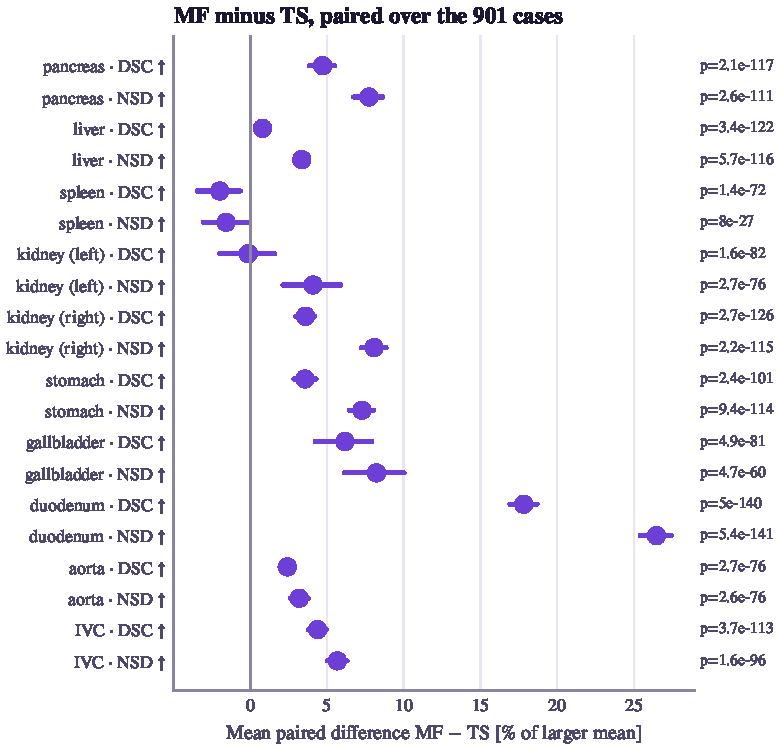
\includegraphics[width=0.76\linewidth]{figures/f_forest.pdf}
\caption{\textbf{Paired differences with 95\% intervals}, as a percentage of the larger mean. Right of zero:
MedFormer's mean is higher.}
\label{fig:forest}
\end{figure}

MedFormer is better in most patients on every organ, including the spleen (\fracSpleenDice\% of patients), where its
\emph{mean} Dice is lower than TotalSegmentator's (\mfSpleenDice{} vs.\ \tsSpleenDice) because of the failure tail
above. The same tail makes MedFormer's mean HD95 worse on \nHDmeanWorse{} of the ten organs, although it has the lower
HD95 in most patients on \nHDmedBetterFrac{} of the ten. With 901 paired patients every difference is significant, so the
fraction of patients and the size of the difference are the informative numbers.

\begin{table}[!htbp]
\centering\small
\caption{\textbf{Ranking the two models with two schemes}, on Dice. Bootstrap $\tau$: median agreement (Kendall's
$\tau$) between the ranking on resampled test sets and the full-data ranking.}
\label{tab:ranking}
% generated by make_report.py
\begin{tabular}{lrlrlr}
\toprule
Structure & mean Dice MF / TS & winner & mean rank MF / TS & winner & bootstrap $\tau$ \\
\midrule
Pancreas & .864 / .823 & MedFormer & 1.09 / 1.91 & MedFormer & 1.00 \\
Liver & .971 / .963 & MedFormer & 1.06 / 1.93 & MedFormer & 1.00 \\
Spleen & .928 / .946 & TotalSegmentator & 1.18 / 1.79 & MedFormer & 1.00 \\
Kidney (left) & .889 / .890 & TotalSegmentator & 1.12 / 1.85 & MedFormer & 1.00 \\
Aorta & .903 / .881 & MedFormer & 1.20 / 1.80 & MedFormer & 1.00 \\
\bottomrule
\end{tabular}

\end{table}

\subsection{Cohorts}

\begin{table}[!t]
\centering\footnotesize\renewcommand{\arraystretch}{1.0}
\caption{\textbf{MedFormer by patient group.} Mean per group of the PanTS metadata (groups under 5 patients and
patients without metadata omitted). \emph{Adjusted $p$}: Kruskal--Wallis or Mann--Whitney test across the groups of a
factor, Holm-corrected over all \nCohTests{} cohort tests. Lesion Dice includes tumour-free patients.}
\label{tab:cohorts}
% generated by make_report.py
\begin{tabular}{llrrrr}
\toprule
Factor & group & $n$ & pancreas Dice & pancreas NSD & lesion Dice \\
\midrule
\multirow{4}{*}{CT phase} & Arterial & 162 & .838 & .832 & .612 \\
 & Delay & 12 & .875 & .847 & .590 \\
 & Non-contrast & 134 & .806 & .776 & .599 \\
 & Venous & 593 & .884 & .878 & .593 \\
 & \emph{adjusted $p$} & & $<\!10^{-3}$ & $<\!10^{-3}$ & 1.000 \\ \midrule
\multirow{3}{*}{Scanner} & GE & 42 & .719 & .695 & .517 \\
 & Philips & 11 & .819 & .752 & .556 \\
 & Siemens & 334 & .850 & .830 & .590 \\
 & \emph{adjusted $p$} & & $<\!10^{-3}$ & 0.004 & 1.000 \\ \midrule
\multirow{7}{*}{Country} & CH & 88 & .832 & .820 & .486 \\
 & CN & 60 & .859 & .830 & .641 \\
 & DE & 182 & .904 & .882 & .575 \\
 & FR & 19 & .908 & .936 & .684 \\
 & TR & 5 & .940 & .980 & .400 \\
 & US & 444 & .850 & .846 & .620 \\
 & multinational & 103 & .875 & .863 & .599 \\
 & \emph{adjusted $p$} & & $<\!10^{-3}$ & $<\!10^{-3}$ & 1.000 \\ \midrule
\multirow{3}{*}{Slice thickness} & $\le$\,1.25 mm & 246 & .793 & .790 & .669 \\
 & 1.25--3 mm & 461 & .890 & .869 & .602 \\
 & $>$\,3 mm & 194 & .894 & .900 & .495 \\
 & \emph{adjusted $p$} & & $<\!10^{-3}$ & $<\!10^{-3}$ & 0.005 \\ \midrule
\multirow{2}{*}{Sex} & F & 222 & .856 & .837 & .546 \\
 & M & 269 & .843 & .830 & .643 \\
 & \emph{adjusted $p$} & & 1.000 & 1.000 & 0.270 \\ \midrule
\multirow{3}{*}{Age} & $<$\,50 & 105 & .872 & .843 & .564 \\
 & 50--65 & 209 & .840 & .822 & .609 \\
 & $>$\,65 & 165 & .863 & .859 & .599 \\
 & \emph{adjusted $p$} & & 1.000 & 1.000 & 1.000 \\ \midrule
\multirow{2}{*}{Tumour} & no tumour & 750 & .859 & .853 & .609 \\
 & tumour & 151 & .889 & .861 & .536 \\
 & \emph{adjusted $p$} & & 1.000 & 1.000 & $<\!10^{-3}$ \\
\bottomrule
\end{tabular}

\end{table}

\noindent\begin{minipage}[c]{0.49\linewidth}\centering
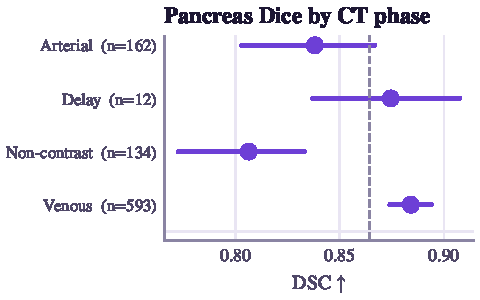
\includegraphics[width=\linewidth]{figures/f_cohort_phase.pdf}
\captionof{figure}{\textbf{Pancreas Dice by CT phase}, mean with 95\% interval (dashed: overall mean).}
\label{fig:cohort}
\end{minipage}\hfill
\begin{minipage}[c]{0.47\linewidth}
Venous-phase scans are segmented best and non-contrast scans worst (adjusted $p$ \cohPhaseP). Thin-slice scans score
\emph{lower} (\cohThin) than thick-slice scans (\cohThick), the opposite of what image resolution alone would
predict, which suggests that slice thickness goes together with differences in site and case mix. These groups are
observational: they point to where to look, not to causes.
\end{minipage}



% ------------------------------------------------------------------
\section{Limitations}
\begin{itemize}
\item \textbf{Not a leaderboard number.} PanTS does not publish its evaluation script, NSD tolerance or detection
  rule; our protocol is documented but may differ from the official one.
\item \textbf{One code fix.} \nPatched{} scans needed a fix of the official padding code (\cref{sec:fix}); without it
  they would have no prediction.
\item \textbf{Empty reference masks.} Some scans have empty reference masks for organs such as the spleen and kidneys;
  we do not know whether the organ is absent, outside the scan or not annotated, and the empty-mask rule scores a
  prediction there as a large error.
\item \textbf{Tumour-free patients} dominate the mean lesion Dice; read the lesion- and patient-level numbers for
  tumours.
\item \textbf{Cohorts are observational}, and some groups are small.
\item \textbf{Only this R-Super checkpoint.} The report-supervised R-Super models and other training settings were not
  evaluated.
\end{itemize}

\section{How to reproduce}
\begin{notebox}
\small
\begin{verbatim}
# official inference (GPU; applies the padding fix) and the comparator
sbatch benchmarks/pants/run_medformer.sbatch
sbatch benchmarks/pants/run_totalseg.sbatch
# evaluation and test-set tables (CPU)
sbatch --export=ALL,MODELS=medformer slurm/pants_eval.sbatch
sbatch --export=ALL,MODELS=totalseg  slurm/pants_eval.sbatch
segevalkit audit --ref data/raw/PanTS/LabelTe --images data/raw/PanTS/ImageTe \
    --workers 16 --out reports/rsuper_medformer/generated/audit_pants_test.csv
python reports/rsuper_medformer/make_report.py   # figures, tables, numbers
tectonic -X compile reports/rsuper_medformer/report.tex
\end{verbatim}
\end{notebox}
Inputs: the per-case results in \texttt{outputs/eval/pants/medformer/} and \texttt{.../totalseg/}, and the test-set
tables in \texttt{outputs/eval/pants/report/}. Code: \url{https://github.com/aj-das-research/SegEvalKit}.

\end{document}
